\chapter{\textsf{\acronym}}
\section*{Descrição}
A \emph{Eurotux Virtualization Appliance} é uma ferramenta de gestão centralizada de recursos disponíveis numa rede. Consiste numa distribuição linux pré-instalada e configurada que permite fazer a gestão via rede de servidores e seus recursos.

O \acronym encontra-se dividido principalmente em dois blocos funcionais:

\begin{itemize}
	\item \emph{Central Management} (CM)
        \item \emph{Virtualization Agent} (VA)
\end{itemize}

\begin{figure}[H]
	\begin{center}
	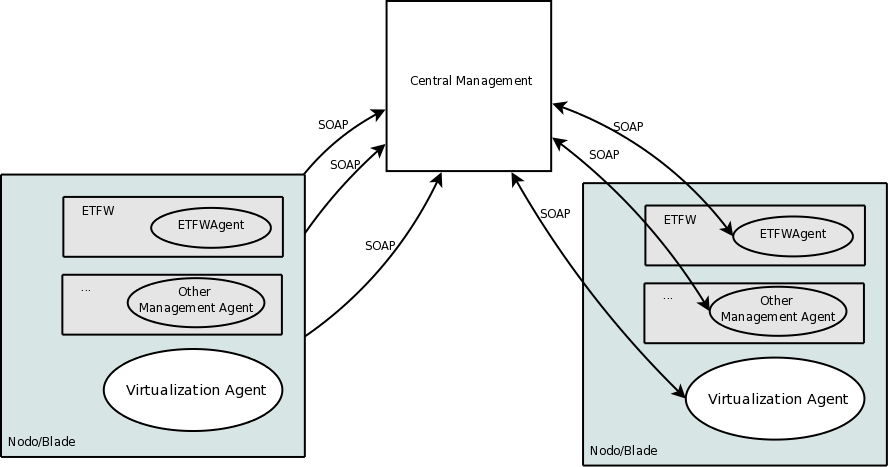
\includegraphics[scale=0.35]{screenshots/etva_blocos.png}
	\caption{Esquema geral do \acronym}
	\label{fig:etva_blocos}
	\end{center}
\end{figure}

O CM é o bloco responsável por gerir toda a infra-estrutura.
Os \emph{Virtualization Agents} são responsáveis pelo processamento dos pedidos entre os servidores de virtualização (\emph{nodes}) e o CM.

Dentro de um servidor de virtualização(\emph{node}) poderão existir máquinas virtuais com \emph{Management Agents}. Estes agentes, permitem a gestão ao nível dos serviços/aplicações instalados numa máquina virtual (ver figura \ref{fig:etva_blocos} ).

Nesta versão em particular, o modelo do \acronym consiste num único servidor de virtualização onde se encontram instalados o CM e o VA. A configuração da rede do \emph{node} neste modelo consiste em quatro interfaces de rede: Internet, LAN, DMZ e Management.
\begin{figure}[H]
    \begin{center}
	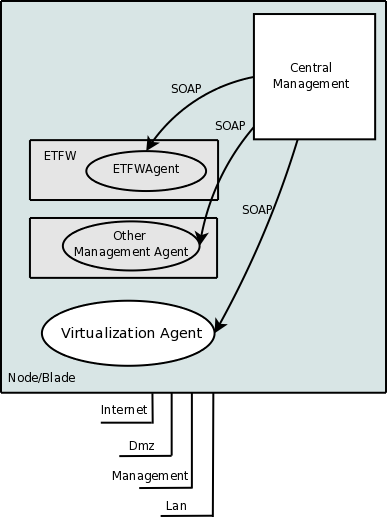
\includegraphics[scale=0.4]{screenshots/etva_standard.png}
	\caption{Modelo \acronym}
	\label{fig:etva_standard}
	\end{center}
\end{figure}
 
Este manual de utilização/configuração descreve a ferramenta de gestão, o CM (\emph{Central Management}).

\pagebreak
\chapter{\textsf{Instalação}}
\label{chp:installation}
\section{Versão standard}

Para efectuar a instalação deveremos ligar a appliance à electricidade, um teclado, um monitor e uma drive CD USB externa.
Depois deverá ser iniciado o boot a partir do cd e teremos a seguinte imagem:

\begin{figure}[H]
	\begin{center}
	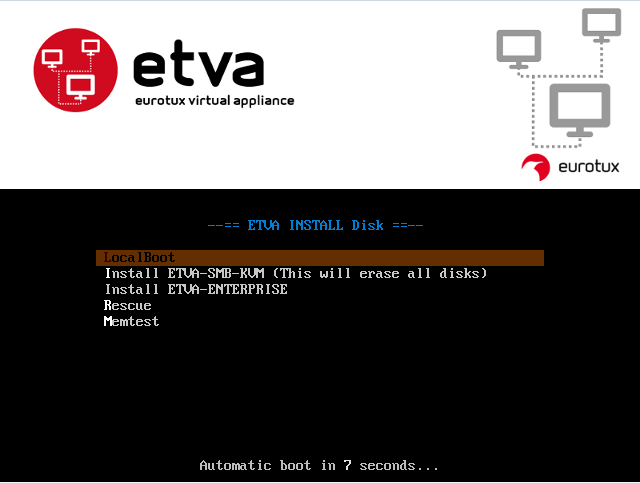
\includegraphics[scale=0.6]{screenshots/install_etva1.png}
	\caption{Menu de instalação da versão ETVA Standard}
	\label{fig:boot_install_screen_standard}
	\end{center}
\end{figure}

De seguida, seleccionando a opção \emph{"Install ETVA-SMB-KVM (This will erase all disks)"} iniciar-se-á o arranque da instalação conforme:

\begin{figure}[H]
	\begin{center}
	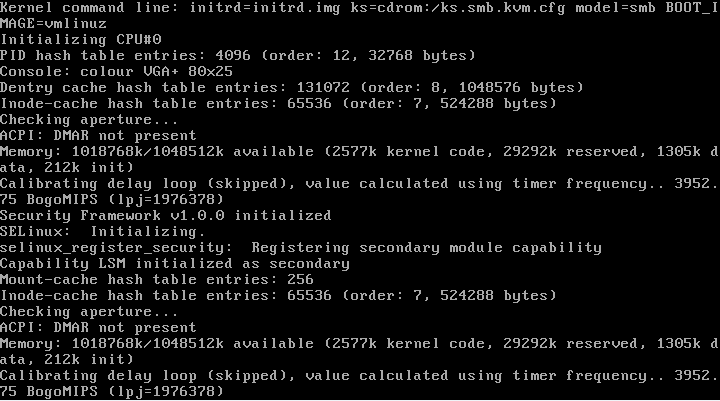
\includegraphics[scale=0.4]{screenshots/install_etva2.png}
    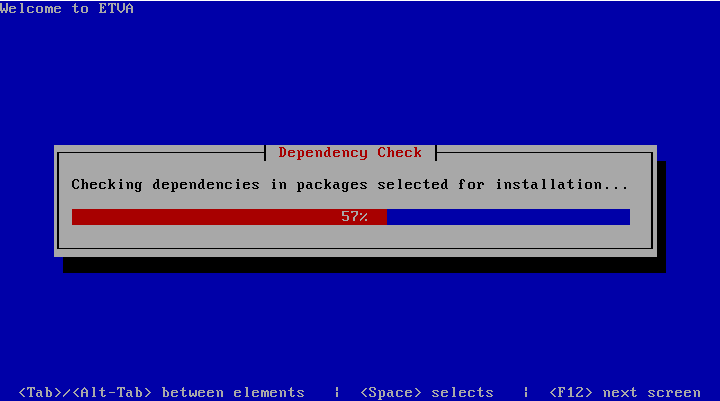
\includegraphics[scale=0.4]{screenshots/install_etva3.png}    
    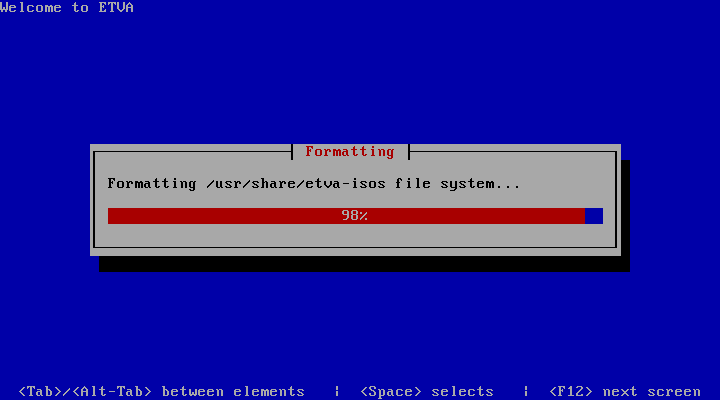
\includegraphics[scale=0.4]{screenshots/install_etva4.png}
    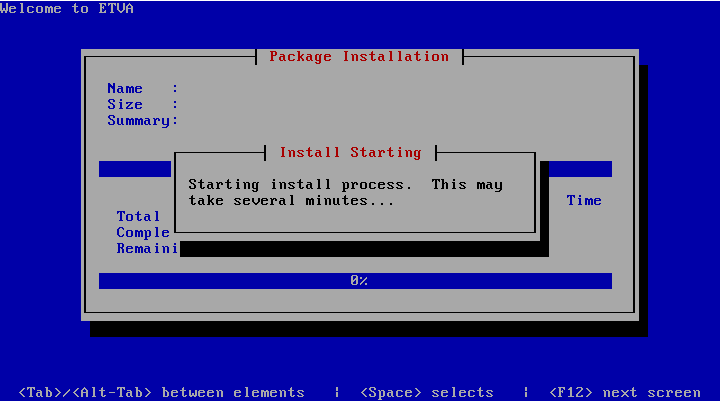
\includegraphics[scale=0.4]{screenshots/install_etva5.png}    
    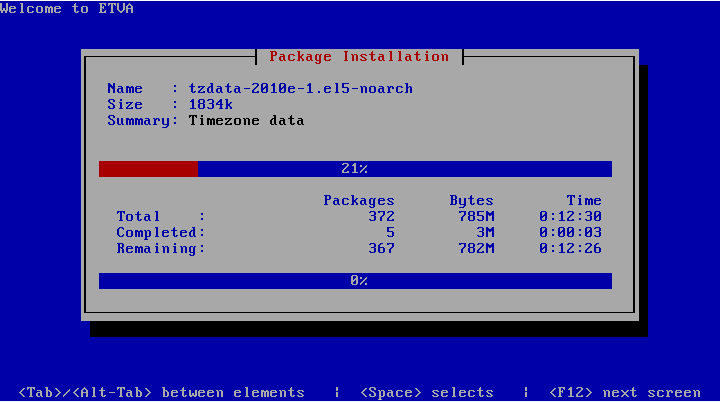
\includegraphics[scale=0.4]{screenshots/install_etva6.png}        
    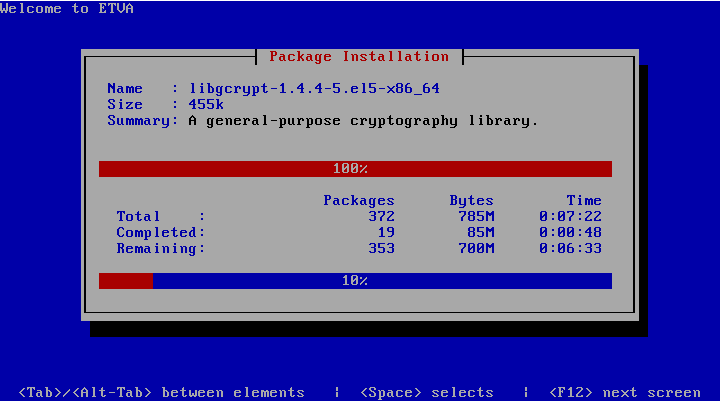
\includegraphics[scale=0.4]{screenshots/install_etva8.png}
    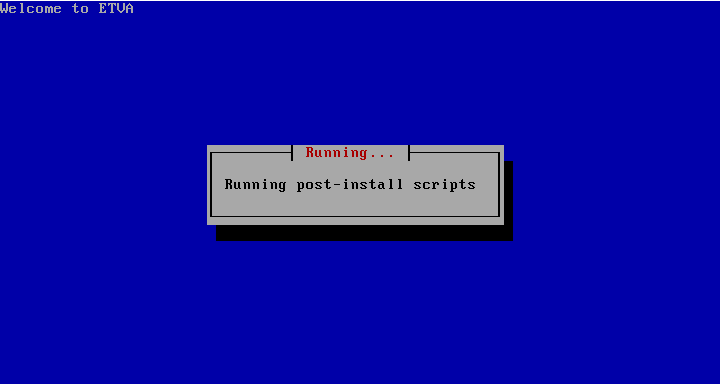
\includegraphics[scale=0.4]{screenshots/install_etva9.png}
    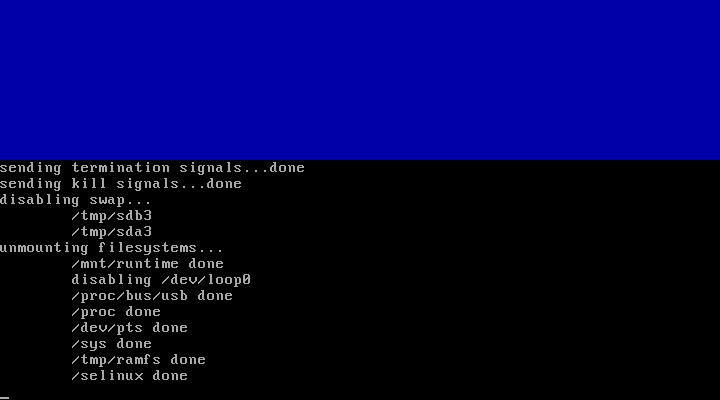
\includegraphics[scale=0.4]{screenshots/install_etva10.png}
\caption{Instação da versão \acronym}
	\label{fig:installation_standard}
	\end{center}
\end{figure}

Depois da instalação efectuada o arranque deverá ser efectuado a partir do disco rígido e deverá aparecer uma imagem como a seguinte:

\begin{figure}[H]
	\begin{center}
	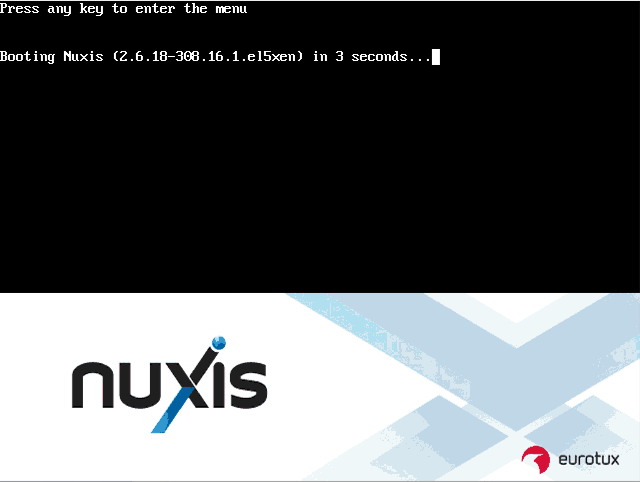
\includegraphics[scale=0.5]{screenshots/install_etva11.png}
	\caption{Menu de boot da versão \acronym}
	\label{fig:boot_screen_standard}
	\end{center}
\end{figure}

No final da instalação deve-se ligar um cabo de rede do nosso PC de acesso à porta \emph{Management} conforme a figura \ref{fig:back_standard}.

\begin{figure}[H]
	\begin{center}
	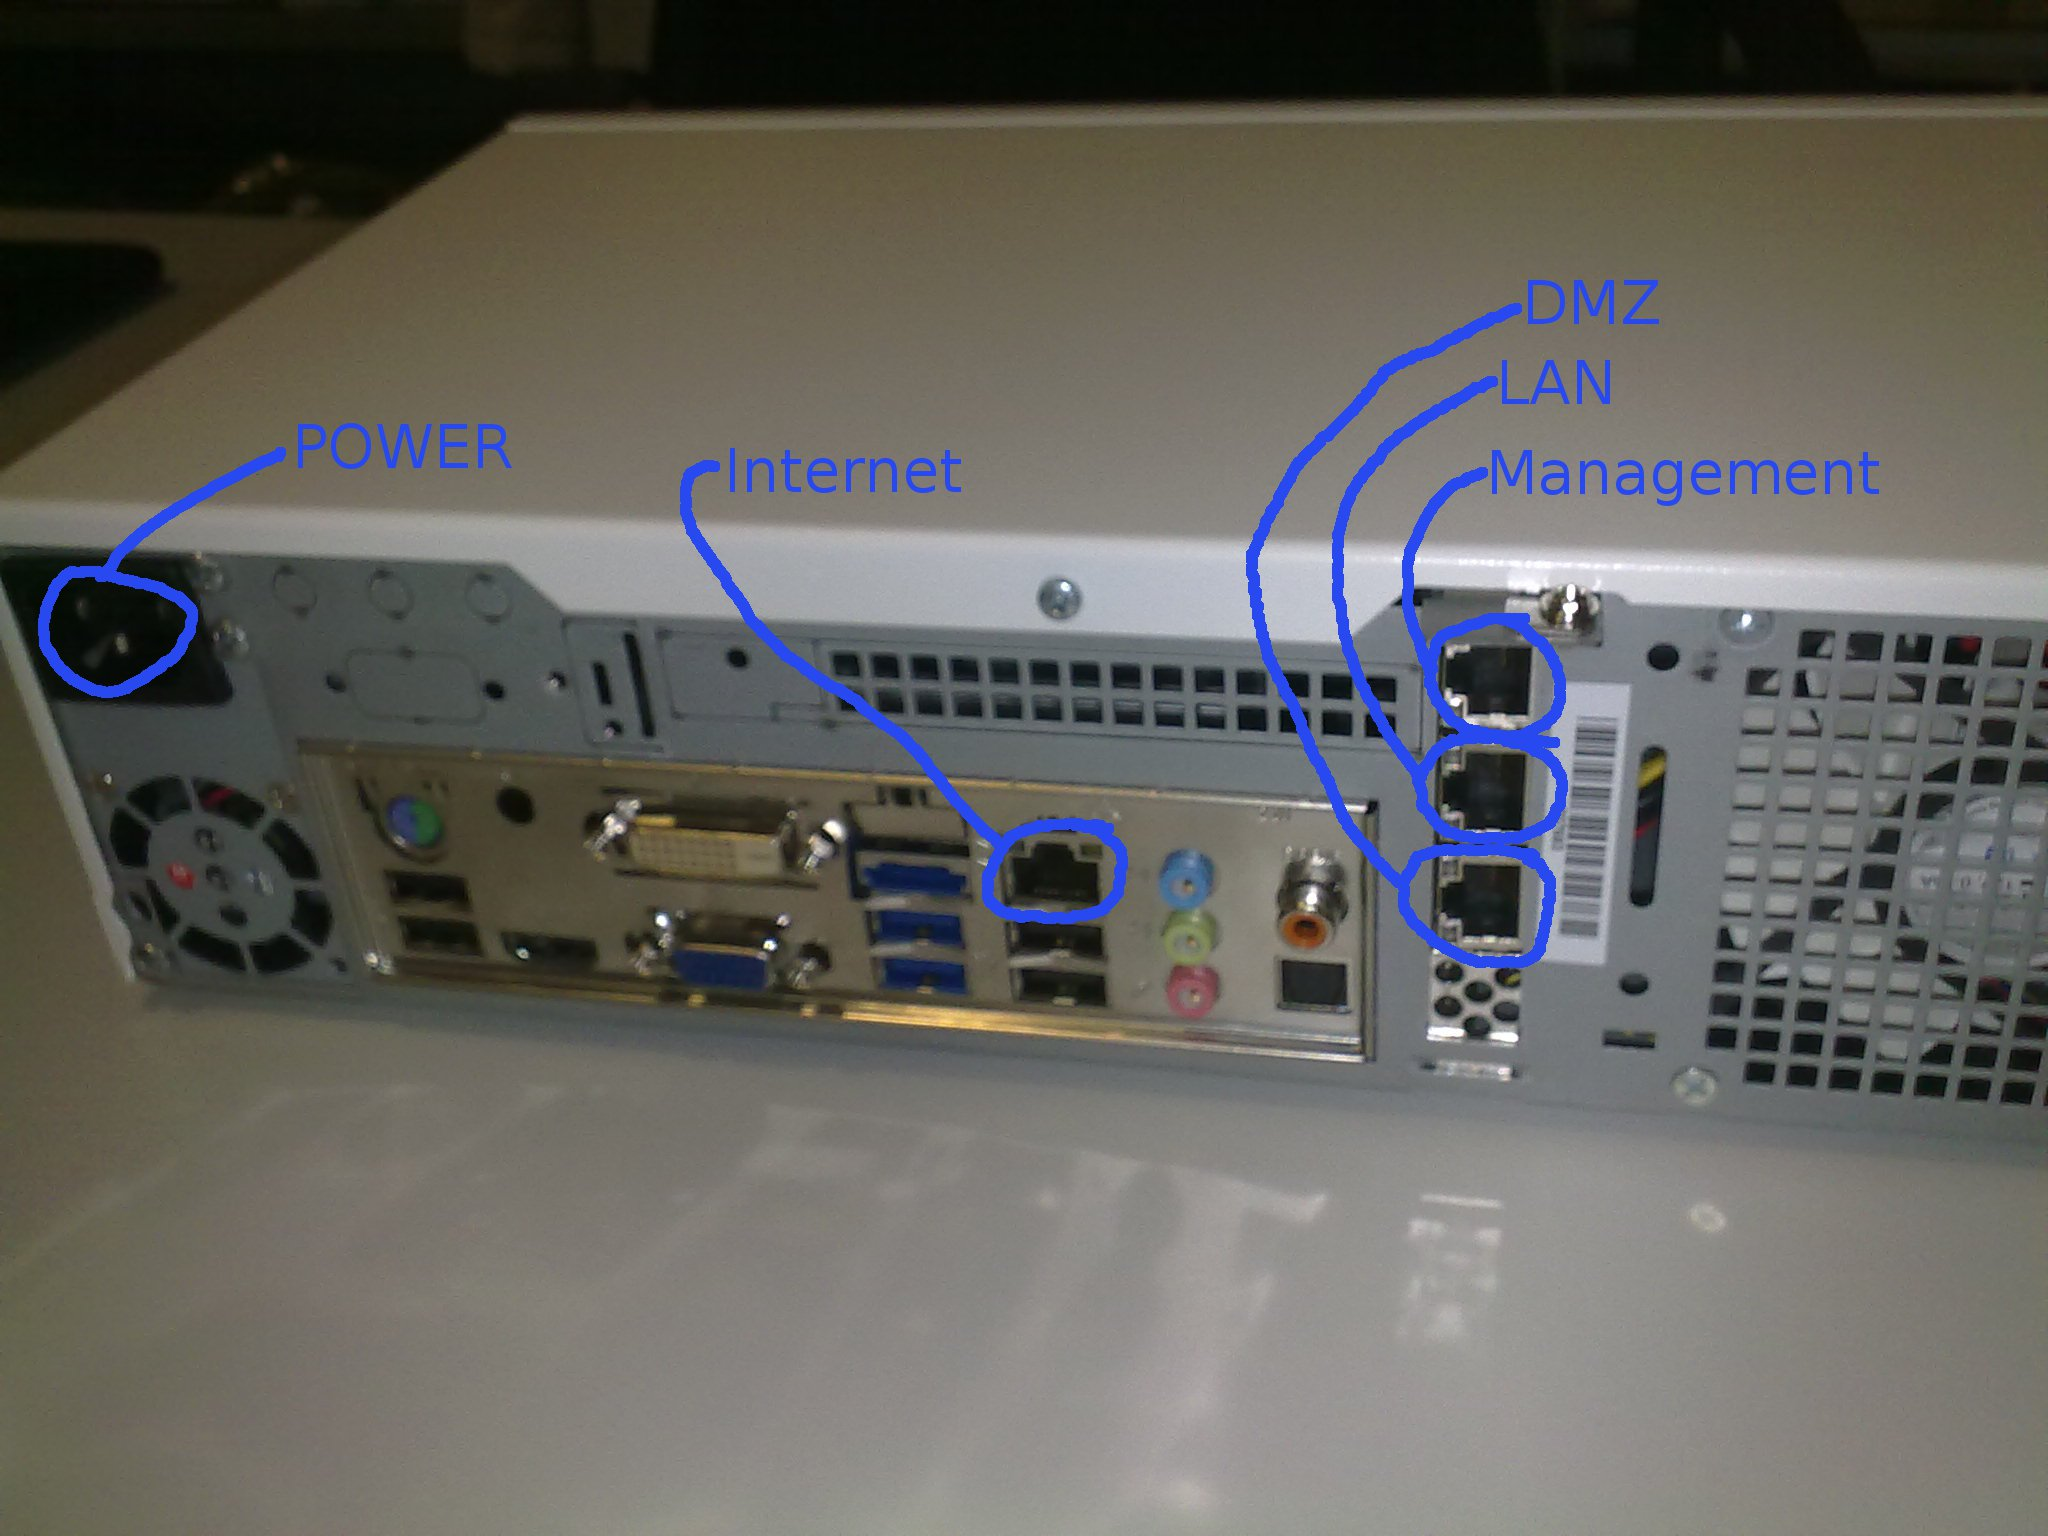
\includegraphics[scale=0.12]{screenshots/appliance_back_identifica.jpg}
	\caption{Identificação das portas a ligar na versão \acronym}
	\label{fig:back_standard}
	\end{center}
\end{figure}

De seguida configura-se a placa de rede do nosso PC:

\begin{quote}
Endereço IP: 10.10.4.1\\
Máscara: 255.255.255.0
\end{quote}

Finalmente, abre-se o nosso browser e acede-se ao seguinte endereço:
\begin{quote}
http://10.10.4.254/
\end{quote}

\pagebreak
